\documentclass[tikz,border=10pt]{standalone}
\begin{document}
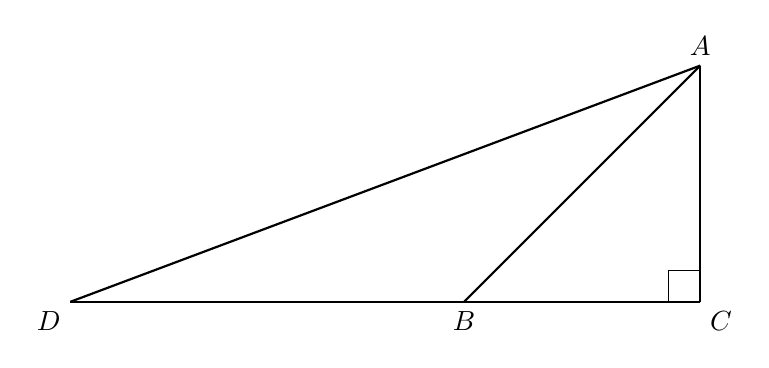
\begin{tikzpicture}
  \coordinate (D) at (0,0);
  \coordinate (B) at (5,0);
  \coordinate (C) at (8,0);
  \coordinate (A) at (8,3);

  \draw[thick] (D) -- (C);
  \draw[thick] (C) -- (A);
  \draw[thick] (D) -- (A);
  \draw[thick] (B) -- (A);

  \draw (7.6,0) -- (7.6,0.4) -- (8,0.4);

  \node[below left] at (D) {$D$};
  \node[below] at (B) {$B$};
  \node[below right] at (C) {$C$};
  \node[above] at (A) {$A$};
\end{tikzpicture}
\end{document}
